\documentclass[../main.tex]{subfiles}

\begin{document}

\section{Feynman diagrammen, processen en correcties}%
\label{sec:feynman_diagrammen_processen_en_correcties}

\subsection{Schrödinger en co}%
\label{sub:schrodinger_en_co}

In de klassieke mechanica hebben we:
\begin{equation}
    \begin{aligned}
        \label{eq:klas_mech}
        \frac{\vec{p}^2}{2m} +V=E
    \end{aligned}
\end{equation}
of voor een vrij deeltje:
\begin{equation}
    \begin{aligned}
        \label{eq:klas_vrij}
        \frac{\vec{p}^2}{2m}=E
    \end{aligned}
\end{equation}
Overgaan naar kwantummechanica geeft:
\begin{equation}
    \begin{aligned}
        \label{eq:kwan_vrij}
        \vec{p}\rightarrow \frac{\vec{\nabla}}{i} \\
        E \rightarrow i \frac{\partial}{\partial t} \\
        - \frac{1}{2m} \vec{\nabla}^2\psi = i \frac{\partial \psi}{\partial t} 
    \end{aligned}
\end{equation}
Relativiteit toevoegen geeft $E^2-\vec{p}^2=m^2$ of in invariante notatie $p^\mu p_\mu-m^2=0$. Vervangen we dit in vergelijking (\ref{eq:kwan_vrij}) krijgen we de Klein-Gordon vergelijkingen.
\begin{equation}
    \begin{aligned}
        \label{eq:klein_gordon}
        -\partial^\mu\partial_\mu \psi - m^2\psi = 0
    \end{aligned}
\end{equation}
Deze zijn door Schrödinger opgesteld voordat hij de Schrödinger vergelijking heeft opgesteld. Dit omdat eerst geprobeerd is de vergelijkingen relativistisch op te lossen, maar dit lukte niet en zijn dan eerst klassiek opgelost. Het probleem bij de Klein-Gordon vergelijkingen is dat $|\psi|^2$ geen probabiliteit meer is a.k.a deze is niet positief definiet. De reden hiervoor is de tweede afgeleide naar de tijd. Dit komt er fysisch op neer dat deeltjes kunnen gecreëerd en geannihileerd kunnen worden. Schrijven we de Klein-Gordon vergelijking eenvoudiger:
\begin{equation}
    \begin{aligned}
        \label{eq:klein_gordon_eenvoudig_1}
        \frac{\partial^2 \psi}{\partial t^2} = \vec{\nabla}^2 \psi - m^2 \psi
    \end{aligned}
\end{equation}
vermenigvuldig dit met de canonische $\psi^*$ en trek er het canonische toegevoegde van af.
\begin{equation}
    \begin{aligned}
        \label{eq:klein_gordon_eenvoudig_2}
        \psi^*\frac{\partial^2 \psi}{\partial t^2} - \psi\frac{\partial^2 \psi^*}{\partial t^2} = \psi^*(\vec{\nabla}^2 \psi - m^2 \psi) - \psi(\vec{\nabla}^2 \psi^* - m^2 \psi^*)
    \end{aligned}
\end{equation}
Dit kan herschreven worden als volgt:
\begin{equation}
    \begin{aligned}
        \label{eq:klein_gordon_eenvoudig_3}
        \frac{\partial}{\partial t} \left(\psi^*\frac{\partial \psi}{\partial t} - \psi\frac{\partial \psi^*}{\partial t}\right) = \vec{\nabla} \cdot §(\psi^*\vec{\nabla} \psi - \psi\vec{\nabla} \psi^*)
    \end{aligned}
\end{equation}
Zo krijgen we iets dat afgeleid is naar de tijd dat moet gelijk zijn aan iets afgeleid naar de ruimte. Dit kan niets anders dan een continuïteit vergelijking.
\begin{equation}
    \begin{aligned}
        \label{eq:continuiteit_vergelijking}
        \frac{\partial \rho}{\partial t} + \vec{\nabla} \cdot \vec{J} &= 0\\
        \rho &= i\left(\psi^*\frac{\partial \psi}{\partial t} - \psi\frac{\partial \psi^*}{\partial t}\right)
    \end{aligned}
\end{equation}
Voor een vrij deeltje (plane wave) is de golffunctie:
\begin{equation}
    \begin{aligned}
        \label{eq:golffunctie_vrij}
        \psi(\vec{x}, t) = Ne^{i(\vec{p}\cdot \vec{x}-Et)}
    \end{aligned}
\end{equation}
met $N$ de normalisatieconstante. Vul dit in $\rho$ in en krijgen we:
\begin{equation}
    \begin{aligned}
        \label{eq:dens_vrij}
        \rho &= 2|N|^2E\\
        E&=\pm\sqrt{p^2+m^2}
    \end{aligned}
\end{equation}
Belangrijk hier is dat $E$ niet constant is en dus ook de densiteit aan deeltjes is niet constant. De $E$ in de relativiteit komt van de Lorentz contractie. Naarmate de energie toeneemt zal door de normalisatie van de golfvergelijking het volume kleiner worden.

\subsection{Dirac}%
\label{sub:dirac}

Dirac wil de kwantummechanica en relativiteit toch samenvoegen. Hij zoekt naar een vergelijking die eerste orde is in $t$.
\begin{equation}
    \begin{aligned}
        \label{eq:dirac_vergelijking}
        \hat E \psi = (\vec{\alpha} \cdot \hat{p} + \beta m)\psi
    \end{aligned}
\end{equation}
En hij eist dat $\psi$ voldoet aan de Klein-Gordon vergelijkingen. Zo gaan de niet te interpreteren densiteiten $\rho$ weg. De enige manier om dit op te lossen is wanneer $\vec{\alpha}$ en $\beta$ 4 $\times$ 4 matrices zijn. Dit omdat er aan anti-commutatie relaties zal moeten voldaan worden, wat niet kan met getallen. Dit geeft mee dat $\psi$ 4 componenten zal hebben, ``Dirac spinor''.
\begin{equation}
    \begin{aligned}
        \label{eq:dirac_spinor}
        \psi(x)=
        \begin{pmatrix}
            \psi_1\\
            \psi_2\\
            \psi_3\\
            \psi_4
        \end{pmatrix}
        =
        \begin{pmatrix}
            \phi\\
            \chi
        \end{pmatrix}
    \end{aligned}
\end{equation}
\begin{equation}
    \begin{aligned}
        \label{eq:dirac_beta}
        \beta=
        \begin{pmatrix}
            I & 0\\
            0 & -I
        \end{pmatrix}
    \end{aligned}
\end{equation}
\begin{equation}
    \begin{aligned}
        \label{eq:dirac_alpha}
        \alpha_i=
        \begin{pmatrix}
            0 & \sigma_i\\
            \sigma_i & 0
        \end{pmatrix}\\
        \sigma_x=
        \begin{pmatrix}
            0 & 1\\
            1 & 0
        \end{pmatrix}\\
        \sigma_y=
        \begin{pmatrix}
            0 & -i\\
            i & 0
        \end{pmatrix}\\
        \sigma_z=
        \begin{pmatrix}
            1 & 0\\
            0 & -1
        \end{pmatrix}\\
    \end{aligned}
\end{equation}
Nu is het mogelijk om de Dirac vergelijking (vergelijking (\ref{eq:dirac_vergelijking})) te herschrijven in zijn covariante vorm:
\begin{equation}
    \begin{aligned}
        \label{eq:dirac_covariant}
        i\gamma^\mu\partial_\mu\psi - m\psi =0
    \end{aligned}
\end{equation}

met $\gamma$ de eerder gedefineerde 4$\times$4 matrices genormeerd naar de lichtsnelheid.

\subsection{Spin}%
\label{sub:spin}

Het probleem dat Dirac vaststelt is dat het angulaire momentum $\vec{L}=\vec{r}\times\vec{p}$ niet zal behouden worden in de relativistische kwantummechanica maar wel in de klassieke kwantummechanica.

\begin{table}[h]
    \centering
    \caption{caption}
    \label{tab:rel_vs_klas_kwan}
    \begin{tabular}{l|l|l}
        $\hat{H}_{SE} = \frac{\hat{\vec{p}}^2}{2m}$             & $[\hat{H},\hat{\vec{L}}]=0$                           & $L$ conserved \\
        $\hat{H}_D = \vec{\alpha}\cdot \hat{\vec{p}}+\beta m$   & $[\hat{H},\hat{\vec{L}}]=-i\vec{\alpha}\cdot \vec{p}$ & $L$ not conserved
    \end{tabular}
\end{table}

In plaats van op te geven gaat hij kijken naar
\begin{equation}
    \begin{aligned}
        \label{eq:dirac_S}
        \hat{S}_i \equiv \frac{1}{2} \hat{\sum}_i \equiv \frac{1}{2}
        \begin{pmatrix}
            \sigma_i & 0 \\
            0 & \sigma_i
        \end{pmatrix}
    \end{aligned}
\end{equation}
waarbij bewezen kan worden dat $[\hat{H}_D,\hat{\vec{S}}]=+i\vec{\alpha}\times\vec{p}$ is.
\begin{equation}
    \begin{aligned}
        \label{eq:bewijs_H_S_1}
        [\hat{H}_D,\hat{\vec{S}}] &= [\vec{\alpha}\times\vec{p},\hat{\vec{S}}] +m[\beta, \hat{\vec{S}}]
    \end{aligned}
\end{equation}
De spin zal niet interagreren met $\beta$ en de commutatierelatie nul.
\begin{equation}
    \begin{aligned}
        \label{eq:bewijs_H_S_2}
        [\hat{H}_D,\hat{\vec{S}}] &= [\vec{\alpha}\times\vec{p},\hat{\vec{S}}]
    \end{aligned}
\end{equation}
Aan de hand van Lie algebra zien we direct dat deze commutatie neerkomt op
\begin{equation}
    \begin{aligned}
        \label{eq:bewijs_H_S_2}
        [\hat{H}_D,\hat{\vec{S}}] &= i\vec{\alpha} \times \vec{p}
    \end{aligned}
\end{equation}
Voegen we dit allemaal samen kunnen we zien dat het totaal angulair momentum we zal behouden worden.
\begin{equation}
    \begin{aligned}
        \label{eq:H_J}
        [\hat{H}_D,\hat{\vec{J}}] = [\hat{H}_D,\hat{\vec{L}}+\hat{\vec{S}}] = 0
    \end{aligned}
\end{equation}
Uit de Dirac vergelijkingen kunnen we direct halen dat de spin van deze deeltjes $\frac{1}{2}$ zijn en dat de Dirac deeltjes dus fermionen zijn.\\
Vullen we in vergelijking (\ref{eq:dirac_covariant}) de golffunctie in voor het vrije deeltje in:
\begin{equation}
    \begin{aligned}
        \label{eq:dirac_vrij_golf}
        \psi(\vec{x},t)=(u(E,\vec{p})e^{i(\vec{p}\cdot\vec{x} -Et)}
    \end{aligned}
\end{equation}
dan krijgen we met de vereenvoudigde dirac vergelijking
\begin{equation}
    \begin{aligned}
        \label{eq:dirac_vrij}
        (\gamma_\mu p^\mu-m)u=0
    \end{aligned}
\end{equation}
4 oplossingen:
\begin{equation}
    \begin{aligned}
        \label{eq:dirac_vrij_opl}
        u^{(1)}=
        \begin{pmatrix}
            1\\
            0\\
            \frac{p_z}{E+m}\\
            \frac{p_x+i_{p_y}}{E+m} 
        \end{pmatrix},
        u^{(2)}=
        \begin{pmatrix}
            1\\
            0\\
            \frac{p_x-i_{p_y}}{E+m} 
            \frac{-p_z}{E+m}\\
        \end{pmatrix},
    \end{aligned},
        u^{(3)},u^{(4)}
\end{equation}
en hun energie:
\begin{equation}
    \begin{aligned}
        \label{eq:dirac_vrij_energie}
        u^{(1)}(u^{(2)}):E=+|\sqrt{p^2+m^2}|\\
        u^{(3)}(u^{(4)}):E=-|\sqrt{p^2+m^2}|\\
    \end{aligned}
\end{equation}
De negatieve energieën kunnen geïnterpreteerd worden als de
\begin{itemize}
    \item negatieve energie deeltje terug gaande in de tijd
    \item positieve energie anti-deeltje voorwaarts in de tijd
\end{itemize}
{\color{green} Na verder inzien lijkt het me niet nuttig om de dirac vergelijkingen verder uit te schrijven hier. Deze staan perfect uitgewerkt in Thomson. Voor dit deel schrijf ik enkel belangrijke mededelingen neer uit de les.}

\subsection{Spin toestanden}%
\label{sub:spin_toestanden}

De heliciteit is niet triviaal voor een bewegend deeltje. Om dit te definiëren maken we gebruik van de heliciteit:
\begin{equation}
    \begin{aligned}
        \label{eq:heliciteit}
        h \equiv \frac{\vec{S}\cdot\vec{p}}{p} 
    \end{aligned}
\end{equation}
We doen dit omdat de z-as natuurlijk niet Lorentz invariant is. Door de spin te projecteren op het momentum van het deeltje wat natuurlijk wel invariant is wordt dit probleem opgelost. De deeltjes hebben dus zowel een spin als heliciteit met de heliciteit enerzijds parallel (rechts handig) of antiparallel (links handig) aan het momentum van het deeltje. Belangrijk om te weten is dat heliciteit nog steeds niet Lorentz invariant is.

\subsection{Intrinsieke pariteit}%
\label{sub:intrinsieke_pariteit}

Ik verwijs hier terug naar de Thomson p. 108. De uitkomsten voor de pariteit operator
\begin{equation}
    \begin{aligned}
        \label{eq:dirac_par_op}
        x'=-x\\
        y'=-y\\
        z'=-z\\
        \psi'=\hat{P}\psi\\
        \hat{P}\psi'=\psi
    \end{aligned}
\end{equation}
zijn gegeven door:
\begin{equation}
    \begin{aligned}
        \label{eq:dirac_int_par}
        i\gamma^1 \frac{\partial \psi}{\partial x} + i\gamma^2 \frac{\partial \psi}{\partial y} + i\gamma^3 \frac{\partial \psi}{\partial z} - m\psi &= -i\gamma^0 \frac{\partial \psi}{\partial t}\\
        i\gamma^1 \frac{\partial \psi'}{\partial x'} + i\gamma^2 \frac{\partial \psi'}{\partial y'} + i\gamma^3 \frac{\partial \psi'}{\partial z'} - m\psi' &= -i\gamma^0 \frac{\partial \psi'}{\partial t}\\
    \end{aligned}
\end{equation}
Hieruit kunnen we halen dat $\gamma^0\hat{P} \propto I$ en dat $\hat{P}^2=I$. Dit wetende bekomen we dat $\hat{P}=\pm\gamma^0$. We hebben dus keuze welke operator we gebruiken. Conventioneel kiezen we $\hat{P}=+\gamma^0$ zodat
\begin{equation}
    \begin{aligned}
        \label{eq:par_u_v}
        \hat{P}u_{1,2} &= +u_{1,2}\\
        \hat{P}v_{1,2} &= -v_{1,2}\\
    \end{aligned}
\end{equation}
Ryckbosch legt hier vooral de nadruk op de fysische concepten en niet op de wiskunde.

\subsection{Spinoren}%
\label{sub:spinoren}

De adjunct spinor is gegeven door
\begin{equation}
    \begin{aligned}
        \label{eq:adj_dirac_spinor}
        \overline \psi = \psi^\dagger\gamma^0 =
        \begin{pmatrix}
            \psi_1^* & \psi_2^* & -\psi_3^* & -\psi_4^*
        \end{pmatrix}
    \end{aligned}
\end{equation}
$\overline \psi \psi$ is Lorentz invariant de stroom is gegeven door $j^\mu = \overline \psi ^\mu \psi$ en de densiteit $\rho = \psi^\dagger\psi = 2E$.

\subsection{Fermi's gouden regel}%
\label{sub:fermi_s_gouden_regel}

Nemen we een hamiltoniaan $\hat{H}_0\phi_k=E_k\phi_k$ en laat deze perturberen met de interactie hamiltoniaan $\hat{H}'(\vec{x},t)$ dan krijgen we volgens de gouden regel dat de Schrödinger vergelijking aanpast naar
\begin{equation}
    \begin{aligned}
        \label{eq:fermi_pert}
        i \frac{d\psi}{dt} = [\hat{H}_0 + \hat{H}'(\vec{x},t)]\psi
    \end{aligned}
\end{equation}
Het is mogelijk om hieruit te bewijzen (zie Thomson p. 51 en verder, Interesseert Ryckbosch minder) dat de breedte van toestand $i$ naar toestand $f$ gegeven is door
\begin{equation}
    \begin{aligned}
        \label{eq:fermi_gouden_regel}
        \Gamma_{fi}=2\pi|T_{fi}|^2\rho(E_i)
    \end{aligned}
\end{equation}
Hierbij zijn
\begin{equation}
    \begin{aligned}
        \label{eq:fermi_par}
        T_{fi}=\left<f|\hat{H}'|i\right> &= \int \phi_f^*(\vec{x})\hat{H}'\phi_f(\vec{x})d^3\vec{x}\quad \text{(Eerste orde storing)}\\
                                         &= \left<f|\hat{H}'|i\right> + \sum_{k\neq i} \frac{\left<f|\hat{H}'|k\right>\left<k|\hat{H}'|i\right>}{E_i-E_k}\quad \text{(Tweede orde s.r.)}\\
        \rho(E_i)&=\left| \frac{dn}{dE_f} \right|_{E_i}
    \end{aligned}
\end{equation}
In deze cursus gaat het vooral over de tweede orde storingsrekening gaan, vanwege 1 intermediare toestand.

\subsection{Faseruimte}%
\label{sub:faseruimte}

Uit de gouden regel van Fermi kunnen we halen dat elke kwantumtoestand in de impulsruimte een volume van $(2\pi)^3$ zal innemen (Heisenberg).
\begin{equation}
    \begin{aligned}
        \label{eq:fermi_faseruimte}
        d^3\vec{x}d^3\vec{p} = (2\pi)^3
    \end{aligned}
\end{equation}
Hierbij is $d^3\vec{x}$ het volume en kunnen we $d^3\vec{p}$ afleiden. Bij dit afleiden gaan we ervan uit dat deze isotroop is verdeeld.
\begin{equation}
    \begin{aligned}
        \label{eq:fermi_aantal_deeltjes}
        dn=4\pi p^2dp\times \frac{V}{(2\pi)^3} 
    \end{aligned}
\end{equation}
Door het normeren van de golffuncties in vergelijking (\ref{eq:fermi_par}) zal in de werkzame doorsnede het volume van de ruimte geen rol meer spelen. De $p^2dp$ zal ons vertellen hoe gemakkelijk een transitie zal gebeuren en is dus zeer belangrijk. Een voorbeeld hiervan is gegeven door het muon verval
\begin{equation}
    \begin{aligned}
        \label{eq:muon_verval}
        \mu \rightarrow e+\nu_e + \nu_\mu
    \end{aligned}
\end{equation}
Het muon heeft een energie van 105MeV en vervalt in 3 deeltjes. Er zijn dus 2 vrijheidsgraden (behoud energie en impuls), $p_1$ en $p_2$. De breedte wordt dan
\begin{equation}
    \begin{aligned}
        \label{eq:breedte_muon}
        \Gamma &\sim \int p_1^2 p_2^2 dp_1 dp_2\\
               &\sim [E]^5\\
               &\Downarrow\\
        \Gamma_\mu &\sim m_\mu^5
    \end{aligned}
\end{equation}
Daarentegen vervalt een top quark enkel naar 2 deeltjes en heeft dus maar 1 vrijheidsgraad $p$.
\begin{equation}
    \begin{aligned}
        \label{eq:top_verval}
        t&\rightarrow b+W\\
        \gamma_t &\sim \int p^2dp\\
                 &\sim m_t^3
    \end{aligned}
\end{equation}
De reden waarom we maar tot de 5de macht krijgen voor het muon en niet tot de 6de is omdat $p_1$ en $p_2$ van elkaar afhangen en een van de 2 integralen weg vallen.\\
Tot nu toe was alles niet relativistisch. Eens we overschakelen naar de relativistische equivalenten wordt alles veel moeilijker. Hier gaan we over op Lorentz invariante fase ruimte en alle problemen worden opgevangen in de normalisatie van de golffuncties. Meer hoeven we hier niet van te weten.

\subsection{Feynman diagrammen}%
\label{sub:feynman_diagrammen}

Een eenvoudig voorbeeld voor feynman diagrammen\\
\begin{minipage}[c]{0.5\textwidth}
    \begin{center}
        \feynmandiagram[horizontal=a to b]{
            a -- [boson, edge label=\(X\)] b,
            i1 -- [fermion, edge label=\(p_1\)] a,
            a -- [fermion, edge label=\(p_2\)] i2,
            f1 -- [fermion, edge label=\(p_3\)] b,
            b -- [fermion, edge label=\(p_4\)] f2,
        };
    \end{center}
\end{minipage}\noindent
\begin{minipage}[c]{0.5\textwidth}
    \begin{center}
        \feynmandiagram[vertical=a to b]{
            a -- [boson, edge label=\(X\)] b,
            i1 -- [fermion, edge label=\(p_1\)] a,
            a -- [fermion, edge label=\(p_2\)] i2,
            f1 -- [fermion, edge label=\(p_3\)] b,
            b -- [fermion, edge label=\(p_4\)] f2,
        };
    \end{center}
\end{minipage}
\begin{equation}
    \begin{aligned}
        \label{eq:fd_voorbeeld}
        \mathcal{M}_{fi}=\left<\psi_c|V|\psi_a\right> \frac{1}{q^2-m_X^2} \left<\psi_d|V|\psi_b\right>
    \end{aligned}
\end{equation}
De makkelijkste vorm van een vertex is als het een scalaire interactie is $\left<\psi_c|V|\psi_a\right> \propto g_a$. Bij de propagaotor zal er moeten gesommeerd worden over alle polarisatie-toestanden. De feynmanregels schrijf ik hier niet helemaal uit, ga hiervoor naar thomson p114 en verder.

\subsection{QED}%
\label{sub:qed}

Hier wordt er enkel gebruik gemaakt van de elektromagnetische wisselwerking. Zie terug Thomson voor de regels. Het is belangrijk om te begrijpen dat de $\frac{1}{q^2}$ in de propagator van QED zal aangeven hoe gemakkelijk zal zijn om een foton van de ene naar de andere kant een impuls $q$ zal meenemen.

\subsection{Currents}%
\label{sub:currents}

De current density is niet meer dan $j^\mu = \overline \psi \gamma^\mu \psi$ wat 4 vectoren zijn. Dit wordt ook wel een bi-linaire vorm genoemd. Omdat $\overline \psi$ en $\psi$ elk bestaan uit 4 componenten bekomen we 16 mogelijke combinaties die we kunnen samennemen.
\begin{table}[h]
    \centering
    \caption{current lineaire combinaties}
    \label{tab:cur_lin_comb}
    \begin{tabular}{rrc}
                                                    & interactie vorm   & aantal componenten    \\
        \hline
        $\overline \psi \psi$                       & scalar            & 1                     \\
        $\overline \psi\gamma^5 \psi$               & pseudoscalar      & 1                     \\
        $\overline \psi\gamma^\mu \psi$             & vector            & 4                     \\
        $\overline \psi\gamma^\mu\gamma^5 \psi$     & pseudovector      & 4                     \\
        $\overline \psi[\gamma^\mu,\gamma^\nu] \psi$& tensor            & 6                     \\
                                                    & totaal            & 16                    \\
    \end{tabular}
\end{table}

\subsection{Zwakke interactie}%
\label{sub:zwakke_interactie}

\begin{figure}[h]
    \centering
    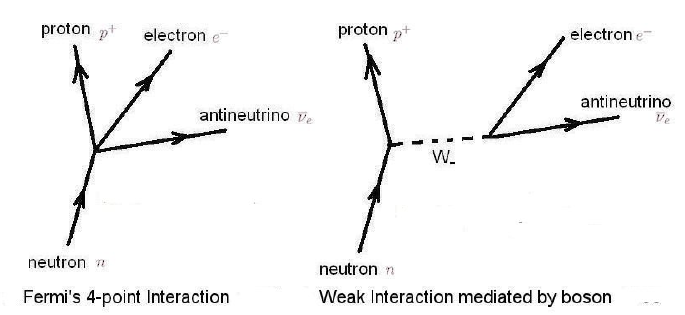
\includegraphics[width=0.8\linewidth]{feynman_diagrams_processes_corrections/zwakke_int.png}
    \caption{Feynman diagram van zwakke interactie}%
    \label{fig:zwakke_int}
\end{figure}

Bij de zwakke interactie wordt er boson uitgewisseld. Eerder werd dit gezien als een puntinteractie. De relatie tussen de 2 is gegeven door
\begin{equation}
    \begin{aligned}
        \label{eq:zwakke_int_const}
        M_F = \frac{G_F}{\sqrt{2}} \overline \psi_{\overline\nu}\gamma_\mu\psi_e\cdot \overline\psi_p\gamma_\mu\psi_n
    \end{aligned}
\end{equation}
Hiet komen we later in de cursus op terug.

\subsection{Charged current}%
\label{sub:charged_current}

Bij het uitwisselen van een $W^+$ of $W^-$ boson wordt er een hoeveelheid lading verplaatst tussen de verschillende deeltjes. Dit kan in principe enkel gebeuren binnen een generatie.
\begin{equation}
    \begin{aligned}
        \label{eq:zwak_gen}
        \begin{pmatrix}
            e^-\\
            \mu^-\\
            \tau^-
        \end{pmatrix}
        &\begin{matrix}
            \leftrightarrow\\
            \leftrightarrow\\
            \leftrightarrow
        \end{matrix}
        \begin{pmatrix}
            \nu_e\\
            \nu_\mu\\
            \nu_\tau
        \end{pmatrix}\\
    \begin{pmatrix}
            u\\
            c\\
            t
        \end{pmatrix}
        &\begin{matrix}
            \leftrightarrow\\
            \leftrightarrow\\
            \leftrightarrow
        \end{matrix}
        \begin{pmatrix}
            d'\\
            s'\\
            b'
        \end{pmatrix}
    \end{aligned}
\end{equation}
Deze opmenging tussen de verschillende generaties is beschreven door de CKM-matrix
\begin{equation}
    \begin{aligned}
        \label{eq:ckm_matrix}
        \begin{pmatrix}
            d'\\
            s'\\
            b'
        \end{pmatrix}
        =
        \begin{pmatrix}
            V_{ud} & V_{us} & V_{ub} \\
            V_{cd} & V_{cs} & V_{cb} \\
            V_{td} & V_{ts} & V_{tb} \\
        \end{pmatrix}
        \begin{pmatrix}
            d\\
            s\\
            b
        \end{pmatrix}
    \end{aligned}
\end{equation}
deze worden ook wel de flavour toestanden (d') en de massa toestanden(d) genoemd.

\subsection{Pariteit schende}%
\label{sub:pariteit_schende}

Uit experimenten bleek dat het heilig boontje, de partiteit, niet behouden wordt bij de zwakke wisselwerking. Later is gezien dat de pariteit volledig zal schenden. De nieuwe theorie die hier is ontwikkeld zegt dat in de operator van de zwakke wisselwerking zowel een vector gedeelte als pseudo-vector gedeelte zit, $P_L= \frac{1}{2} (1-\gamma^5)$ die de links handige toestanden uit projecteerd. Dit geeft de (V-A)-interactie
\begin{equation}
    \begin{aligned}
        \label{eq:v_a_int}
        \frac{1}{2} \overline \psi \gamma^\mu (1-\gamma^5) \phi
    \end{aligned}
\end{equation}
De heliciteit en $P_L$ hier zijn niet helemaal hetzelfde.

\subsection{Neutrale current}%
\label{sub:neutrale_current}

Omdat we $W^\pm$ hebben wil het zeggen dat we een triplet hebben en hebben we dus nog een boson zonder lading nodig, $Z^0$. Deze zal de pariteit maar gedeeltelijk schenden.

\subsection{Mathematical interlude: groups}%
\label{sub:mathematical_interlude_groups}

Een groep is een set van operaties die moeten voldoen aan:
\begin{itemize}
    \item inwendigheid: $R_iR_j$ is ook deel van de set
    \item identiteit: $I$ bestaat met $R_iI = IR_i = R_I$
    \item inversie: $R_I^{-1}$ moet bestaan met $R_I^{-1}R_i=R_iR_I^{-1}=I$
    \item associativiteit: $R_i(J_jR_k)=(R_iR_j)R_k$
    \item commutativiteit: $R_iR_j=R_jR_i$
\end{itemize}
Indien ze hier allemaal aan voldoen is dit een abelse groep. De meest gebruikte in de deeltjes fysica

\begin{table}[h]
    \centering
    \caption{Meest gebruikte groepen}
    \label{tab:deeltjes_groepen}
    \begin{tabular}{ccc}
        Groep &  & Matrices \\
        \hline
        $U(n)$ & $n\times n$ & unitair ($U^*U=1$) \\
        $SU(n)$ & $n\times n$ & unitair, determinant 1 \\
        $O(n)$ & $n\times n$ & orthogonaal ($OO=1$) \\
        $SO(n)$ & $n\times n$ & orthogonaal, determinant 1 \\
    \end{tabular}
\end{table}
De $SO(n)$ groep zijn de rotaties van de ruimte in $n$ dimensies en $SU(2)$ is de spin van deeltjes wat homomorf is met $SO(2)$.

\subsection{2D-rotatie $SO(2)$}%
\label{sub:2d_rotatie_so_2}

Het roteren van de ruimte over een hoek $\phi$ is gegeven door:
\begin{equation}
    \begin{aligned}
        \label{eq:rotatie}
        R(\phi)\hat{e}_1 &= \hat{e}_1 \cos{\phi} + \hat{e}_2 \sin{\phi}\\
        R(\phi)\hat{e}_2 &= -\hat{e}_1 \sin{\phi} + \hat{e}_2 \cos{\phi}\\
        \text{of}\\
        R(\phi)\hat{e}_i &= \hat{e}_jR(\phi)_i^j\\
        R(\phi)&=
        \begin{pmatrix}
            \cos\phi & -\sin\phi\\
            \sin\phi & \cos\phi\\
        \end{pmatrix}
    \end{aligned}
\end{equation}
Laten we dit inwerken op een gewone vector $\vec{x}=\hat{e}_ix^i$ krijgen we:
\begin{equation}
    \begin{aligned}
        \label{eq:rot_vec}
        \vec{x}\rightarrow\vec{x}' &\equiv R(\phi)\vec{x}=R(\phi)\hat{e}_ix^i = \hat{e}_jR(\phi)_i^jx^i\\
        \vec{x}' &= \hat{e}_jx^{'j}\\
        x^{'j}=R(\phi)_i^jx^i
    \end{aligned}
\end{equation}
De verschillende eigenschappen om een abelse groep te bekomen zijn makkelijk na te gaan.\\
Gaan we nog een stap verder , bekijken we de rotatie van infinitisimaal kleine hoeken.
\begin{equation}
    \begin{aligned}
        \label{eq:inf_kleine_rot}
        R(d\phi)=1-id\phi J
    \end{aligned}
\end{equation}
met $J$ onafhankelijk van $d\phi$. De reden voor de vorm van vergelijking (\ref{eq:inf_kleine_rot}) is door de kleine hoek benadering, cos gaat naar 1 en sin gaat naar de hoek zelf. Het bepalen van $J$ kan snel gedaan worden:
Draai de hoek $\phi$ infinitesimaal op:
\begin{equation}
    \begin{aligned}
        \label{eq:bepalen_J_1}
        R(\phi+d\phi) = R(\phi)R(d\phi)=R(\phi)-id\phi R(\phi)J
    \end{aligned}
\end{equation}
Of in taylor ontwikkeling:
\begin{equation}
    \begin{aligned}
        \label{eq:bepalen_J_2}
        R(\phi+d\phi) = R(\phi)+d\phi \frac{dR(\phi)}{d\phi}
    \end{aligned}
\end{equation}
Stel deze gelijk aan elkaar om een vergelijking voor $R(\phi)$ te bekomen.
\begin{equation}
    \begin{aligned}
        \label{eq:bepalen_J_3}
        \frac{dR(\phi)}{d\phi} &= -iR(\phi)J\\
        \Rightarrow R(\phi) &= e^{-i\phi J}
    \end{aligned}
\end{equation}
$J$ is dus niets anders dan de generator van de $SO(2)$ groep (deze groep heeft er maar 1!). Het expliciet uitrekenen van $J$ geeft
\begin{equation}
    \begin{aligned}
        \label{eq:j_expliciet}
        R(d\phi) &=
        \begin{pmatrix}
            1 & -d\phi \\
            d\phi & 1
        \end{pmatrix}\\
        \Rightarrow J&=
        \begin{pmatrix}
            0 & -i \\
            i & 0
        \end{pmatrix}
    \end{aligned}
\end{equation}

\subsection{3D rotatie $SO(3)$}%
\label{sub:3d_rotatie_so_3}

Deze worden in het algemeen voorgesteld in eulerhoeken $\alpha$, $\beta$ en $\gamma$. Deze rotaties commuteren niet en dit is dus geen abelse groep. Dit zal belangrijke gevolgen hebben. De matrix van deze rotatie is gegeven door
\begin{equation}
    \begin{aligned}
        \label{eq:3d_rot}
        R_3(\psi) =
        \begin{pmatrix}
            \cos\psi & -\sin\psi & 0 \\
            \sin\psi & \cos\psi & 0 \\
            0 & 0 & 1 \\
        \end{pmatrix}\\
        R_2(\psi) =
        \begin{pmatrix}
            \cos\psi & 0 & \sin\psi \\
            0 & 1 & 0 \\
            -\sin\psi & 0 & \cos\psi \\
        \end{pmatrix}\\
        R_1(\psi) =
        \begin{pmatrix}
            1 & 0 & 0 \\
            0 & \cos\psi & -\sin\psi \\
            0 & \sin\psi & \cos\psi \\
        \end{pmatrix}\\
    \end{aligned}
\end{equation}
Wat we wel hebben is dat elke subgroep $R_i$ isomorf is met $SO(2)$.
\begin{equation}
    \begin{aligned}
        \label{eq:iso_so_2}
        R_n(\psi)=e^{-i\psi J_n}
    \end{aligned}
\end{equation}
Dit geeft ons 3 generatoren voor de $SO(3)$ groep. Dit kan veralgemeend worden tot: $SU(n)$ heeft $n^2-1$ generatoren.

\subsection{Non-abelse interacties}%
\label{sub:non_abelse_interacties}

Enkel de elektromagnetische wisselwerking is Abels. Al de andere krachten zijn dit niet. De intermediare toestanden van deze niet Abelse interacties zullen zelf hun lading dragen. Hierdoor is het mogelijk dat deze aan zelf-interactie gaan doen.\\
De reden voor de korte dracht van de sterke en zwakke wisselwerking zijn niet hetzelfde. Bij de zwakke wisselwerking ligt dit aan de grote massa van het W en Z boson die snel vervallen. Bij de sterke wisselwerking is dit door de zelf-interactie tussen gluonen.

\end{document}
